\documentclass[journal,12pt,twocolumn]{IEEEtran}
%
\usepackage{setspace}
\usepackage{gensymb}
%\doublespacing
\singlespacing

%\usepackage{graphicx}
%\usepackage{amssymb}
%\usepackage{relsize}
\usepackage[cmex10]{amsmath}
%\usepackage{amsthm}
%\interdisplaylinepenalty=2500
%\savesymbol{iint}
%\usepackage{txfonts}
%\restoresymbol{TXF}{iint}
%\usepackage{wasysym}
\usepackage{amsthm}
%\usepackage{iithtlc}
\usepackage{mathrsfs}
\usepackage{txfonts}
\usepackage{stfloats}
\usepackage{bm}
\usepackage{cite}
\usepackage{cases}
\usepackage{subfig}
%\usepackage{xtab}
\usepackage{longtable}
\usepackage{multirow}
%\usepackage{algorithm}
%\usepackage{algpseudocode}
\usepackage[utf8]{inputenc}
\usepackage{tikz}
\usetikzlibrary{positioning}
\usepackage{enumitem}
\usepackage{mathtools}
\usepackage{steinmetz}
\usepackage{tikz}
\usepackage{circuitikz}
\usepackage{verbatim}
\usepackage{tfrupee}
\usepackage[breaklinks=true]{hyperref}
%\usepackage{stmaryrd}
\usepackage{tkz-euclide} % loads  TikZ and tkz-base
%\usetkzobj{all}
\usetikzlibrary{calc,math}
\usepackage{listings}
    \usepackage{color}                                            %%
    \usepackage{array}                                            %%
    \usepackage{longtable}                                        %%
    \usepackage{calc}                                             %%
    \usepackage{multirow}                                         %%
    \usepackage{hhline}                                           %%
    \usepackage{ifthen}                                           %%
  %optionally (for landscape tables embedded in another document): %%
    \usepackage{lscape}     
\usepackage{multicol}
\usepackage{chngcntr}
%\usepackage{enumerate}

%\usepackage{wasysym}
%\newcounter{MYtempeqncnt}
\DeclareMathOperator*{\Res}{Res}
%\renewcommand{\baselinestretch}{2}
\renewcommand\thesection{\arabic{section}}
\renewcommand\thesubsection{\thesection.\arabic{subsection}}
\renewcommand\thesubsubsection{\thesubsection.\arabic{subsubsection}}

\renewcommand\thesectiondis{\arabic{section}}
\renewcommand\thesubsectiondis{\thesectiondis.\arabic{subsection}}
\renewcommand\thesubsubsectiondis{\thesubsectiondis.\arabic{subsubsection}}

% correct bad hyphenation here
\hyphenation{op-tical net-works semi-conduc-tor}
\def\inputGnumericTable{}                                 %%

\lstset{
%language=C,
frame=single, 
breaklines=true,
columns=fullflexible
}
%\lstset{
%language=tex,
%frame=single, 
%breaklines=true
%}

\begin{document}
%


\newtheorem{theorem}{Theorem}[section]
\newtheorem{problem}{Problem}
\newtheorem{proposition}{Proposition}[section]
\newtheorem{lemma}{Lemma}[section]
\newtheorem{corollary}[theorem]{Corollary}
\newtheorem{example}{Example}[section]
\newtheorem{definition}[problem]{Definition}
%\newtheorem{thm}{Theorem}[section] 
%\newtheorem{defn}[thm]{Definition}
%\newtheorem{algorithm}{Algorithm}[section]
%\newtheorem{cor}{Corollary}
\newcommand{\BEQA}{\begin{eqnarray}}
\newcommand{\EEQA}{\end{eqnarray}}
\newcommand{\define}{\stackrel{\triangle}{=}}
\bibliographystyle{IEEEtran}
%\bibliographystyle{ieeetr}
\providecommand{\mbf}{\mathbf}
\providecommand{\pr}[1]{\ensuremath{\Pr\left(#1\right)}}
\providecommand{\qfunc}[1]{\ensuremath{Q\left(#1\right)}}
\providecommand{\sbrak}[1]{\ensuremath{{}\left[#1\right]}}
\providecommand{\lsbrak}[1]{\ensuremath{{}\left[#1\right.}}
\providecommand{\rsbrak}[1]{\ensuremath{{}\left.#1\right]}}
\providecommand{\brak}[1]{\ensuremath{\left(#1\right)}}
\providecommand{\lbrak}[1]{\ensuremath{\left(#1\right.}}
\providecommand{\rbrak}[1]{\ensuremath{\left.#1\right)}}
\providecommand{\cbrak}[1]{\ensuremath{\left\{#1\right\}}}
\providecommand{\lcbrak}[1]{\ensuremath{\left\{#1\right.}}
\providecommand{\rcbrak}[1]{\ensuremath{\left.#1\right\}}}
\theoremstyle{remark}
\newtheorem{rem}{Remark}
\newcommand{\sgn}{\mathop{\mathrm{sgn}}}
\providecommand{\abs}[1]{\left\vert#1\right\vert}
\providecommand{\res}[1]{\Res\displaylimits_{#1}} 
\providecommand{\norm}[1]{\left\lVert#1\right\rVert}
%\providecommand{\norm}[1]{\lVert#1\rVert}
\providecommand{\mtx}[1]{\mathbf{#1}}
\providecommand{\mean}[1]{E\left[ #1 \right]}
\providecommand{\fourier}{\overset{\mathcal{F}}{ \rightleftharpoons}}
%\providecommand{\hilbert}{\overset{\mathcal{H}}{ \rightleftharpoons}}
\providecommand{\system}{\overset{\mathcal{H}}{ \longleftrightarrow}}
	%\newcommand{\solution}[2]{\textbf{Solution:}{#1}}
\newcommand{\solution}{\noindent \textbf{Solution: }}
\newcommand{\cosec}{\,\text{cosec}\,}
\providecommand{\dec}[2]{\ensuremath{\overset{#1}{\underset{#2}{\gtrless}}}}
\newcommand{\myvec}[1]{\ensuremath{\begin{pmatrix}#1\end{pmatrix}}}
\newcommand{\mydet}[1]{\ensuremath{\begin{vmatrix}#1\end{vmatrix}}}
%\numberwithin{equation}{section}
\numberwithin{equation}{subsection}
%\numberwithin{problem}{section}
%\numberwithin{definition}{section}
\makeatletter
\@addtoreset{figure}{problem}
\makeatother
\let\StandardTheFigure\thefigure
\let\vec\mathbf
%\renewcommand{\thefigure}{\theproblem.\arabic{figure}}
\renewcommand{\thefigure}{\theproblem}
%\setlist[enumerate,1]{before=\renewcommand\theequation{\theenumi.\arabic{equation}}
%\counterwithin{equation}{enumi}
%\renewcommand{\theequation}{\arabic{subsection}.\arabic{equation}}
\def\putbox#1#2#3{\makebox[0in][l]{\makebox[#1][l]{}\raisebox{\baselineskip}[0in][0in]{\raisebox{#2}[0in][0in]{#3}}}}
     \def\rightbox#1{\makebox[0in][r]{#1}}
     \def\centbox#1{\makebox[0in]{#1}}
     \def\topbox#1{\raisebox{-\baselineskip}[0in][0in]{#1}}
     \def\midbox#1{\raisebox{-0.5\baselineskip}[0in][0in]{#1}}
\vspace{3cm}
\title{Matrix Theory: Assignment 5}
\author{Debolena Basak\\ Roll No.: AI20RESCH11003\\ PhD Artificial Intelligence}

\maketitle
\newpage
%\tableofcontents
\bigskip
\renewcommand{\thefigure}{\theenumi}
\renewcommand{\thetable}{\theenumi}


\begin{abstract}
This a problem on tracing a parabola using vector algebra.
\end{abstract}
Download Python code from 
%
\begin{lstlisting}
https://github.com/Debolena/EE5609/blob/master/Assignment_5/parabola%20plot.py
\end{lstlisting}
%
Download all latex-tikz codes from 
%
\begin{lstlisting}
https://github.com/Debolena/EE5609/tree/master/Assignment_5
\end{lstlisting}
%
\section{Problem}
Trace the parabola:
\begin{align}
	(x-4y)^2=51y
\end{align}

\section{Solution}
Expanding the given equation, we have,
\begin{align}
    x^2 -8xy +16y^2 -51y =0 \label{eq:1}
\end{align}
The general equation of second degree is given by
\begin{align}
	ax^2+2bxy+cy^2+2dx+2ey+f=0 \label{gen_eq}
\end{align}
and can be expressed as
\begin{align}
	\vec{x}^T\vec{V}\vec{x}+2\vec{u}^T\vec{x}+f=0 \label{conic_eq}
\end{align}
where
\begin{align}
	\vec{V} &= \vec{V}^T = \myvec{a & b \\ b & c}
	\\
	\vec{u}^T &= \myvec{d & e}
\end{align}
From equation (\ref{eq:1}) , we get
\begin{align}
	\vec{V} &= \myvec{1 & -4\\-4 & 16}\label{eq:2}\\
	\vec{u} &= \myvec{0\\-\frac{51}{2}}\label{eq:3}\\ 
	f &= 0 \label{eq:4}
\end{align}
Expanding the determinant of $\vec{V}$ we observe, 
\begin{align}
	\mydet{1 & -4\\-4 & 16} = 0 \label{eq:4}
\end{align}
Therefore, \ref{eq:1} is a parabola.

The characteristic equation of $\vec{V}$ is given as follows,
\begin{align}
		\mydet{\lambda\vec{I}-\vec{V}} = \mydet{\lambda-1&4\\ 4&\lambda-16} &= 0\\
		\implies \lambda^2-17\lambda &= 0\label{eq:5}
\end{align}
The eigenvalues are given by
\begin{align}
		\lambda_1=0, \lambda_2=17\label{eq:6}    
\end{align}
For $\lambda_1 = 0$, the eigen vector $\vec{p}$ is given by 
\begin{align}
		\vec{V}\vec{p} = 0
\end{align}

Row reducing $\vec{V}$ 
\begin{align}
		\myvec{1&-4\\-4&16}\xleftrightarrow[R_2=R_2+R_1]{R_2=R_2/4}\myvec{1&-4\\0&0}\\
		\implies\vec{p}_1=\frac{1}{\sqrt{17}}\myvec{-4\\-1} \label{eq:7}
\end{align}
Similarly, 
\begin{align}
		\vec{p}_2=\frac{1}{\sqrt{17}}\myvec{-1\\4} \label{eq:8}
\end{align}

Thus,
\begin{align}
		\vec{P}&=\myvec{\vec{p_1}&\vec{p_2}}=\frac{1}{\sqrt{17}} \myvec{-4 & -1\\ -1 & 4} 
\end{align}
The equation of the parabola is:
\begin{align}
		\vec{y^T}\vec{D}\vec{y}&=-2\eta\myvec{1&0}\vec{y}
\end{align}
where
\begin{align}
		\eta=\vec{u}^T\vec{p_1}=\frac{51}{2\sqrt{17}}
\end{align}
and focal length of the parabola is given by 
\begin{align}
	\frac{\abs{2\vec{u}^T\vec{p_1}}}{\lambda_2}	= \frac{3}{\sqrt{17}}
\end{align}

Now,
\begin{align}
		\myvec{\vec{u^T}+\eta\vec{p_1^T} \\ \vec{V}}\vec{c}=
		\myvec{-f \\ \eta\vec{p_1}-\vec{u}} \label{eq:8}
\end{align}
using equations \eqref{eq:2}, \eqref{eq:3} and \eqref{eq:8}
\begin{align}
	\myvec{-6& -27 \\ 1 & -4 \\  -4 & 16 }\vec{c}=\myvec{0 \\ -6\\ 24} 
\end{align}

Forming the augmented matrix and row reducing it:
\begin{align}
		\myvec{-6 & -27 & 0\\1 & -4 & -6 \\-4 & 16 & 24}\\
		\xleftrightarrow[]{R_3\leftarrow R_3+ 4R_2} 
		\myvec{-6 & -27 & 0\\1 & -4 & -6 \\0 & 0 &0 }\\
		\xleftrightarrow[]{R_1\leftarrow R_1/(-6)} 
		\myvec{1 & 9/2 & 0\\1 & -4 & -6\\0 & 0 &0 }\\
		\xleftrightarrow[]{R_2\leftarrow R_2-R_1} 
		\myvec{1 & 9/2 & 0\\0 & -17/2 & -6 \\0 & 0 &0 }\\
		\xleftrightarrow[]{R_2\leftarrow (-\frac{2}{17})R_2}
		\myvec{1 & 9/2 & 0\\0 & 1 & 12/17\\0 & 0 &0}\\ 
		\xleftrightarrow[]{R_1\leftarrow R_1 -(\frac{9}{2})R_2}
		\myvec{1 & 0 & -54/17\\0 & 1 & 12/17 \\0 & 0 &0}
\end{align}

Thus the vertex is:
\begin{align}
	&\vec{c}= \myvec{-\frac{54}{17}\\ \frac{12}{17}} \\
	&\approx \myvec{-3.18\\ 0.71}
\end{align}

\begin{figure}[!htbp]
	\centering
	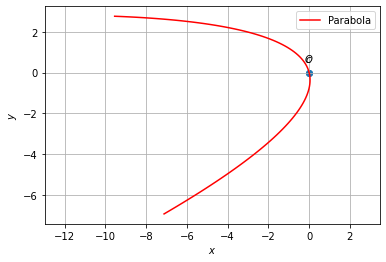
\includegraphics[width =\columnwidth]{parabola plot.png}
	\caption{Parabola }
	\label{fig:1}
\end{figure}	

\end{document}
